\documentclass[12pt]{beamer}
\usepackage[T1]{fontenc}
\usepackage[utf8]{inputenc}
\usepackage{lmodern}
\usepackage[english]{babel}
\usepackage{xcolor}
\usepackage{pgf,tikz}
%\usetikzlibrary{calc}
\usepackage{amssymb,amsmath,array,bm}
\usepackage[T1]{fontenc}
\usepackage[utf8]{inputenc}
\usepackage{hyperref}
\usepackage{multicol}
\usepackage{tabularx}


\def\fnmark#1{{\small}$^#1$}
\def\fnote#1#2{$^#1\;$\texttt{#2}\\}

\usepackage{verbatim}
%\usepackage[active,tightpage]{preview}
\usetheme{Madrid}

\usetikzlibrary{positioning,shapes,shadows,arrows}
\tikzstyle{myarrow}=[<-, >=open triangle 90, thick]
\tikzstyle{line}=[-, thick]

\begin{document}

    \date[SRS'16]{Summer Research School \\ 2016}
    \institute[SHSM]{Sofia High School of Mathematics \\ Sofia, Bulgaria}
    \author[Mr. Kelevedzhiev (BAS), Alex]{
        \begin{table}[]
        \begin{tabular}{rl}
        \normalsize{Author:    } & \normalsize{Alex Ivanov Tsvetanov} \\
        \scriptsize{Mentor:     } & \scriptsize{Emil Kelevedzhiev} \\
        \end{tabular}
        \end{table}
	}
	\title[MEC]{Math Expressions Calculator}

	\begin{frame}
		\titlepage
	\end{frame}

	\begin{frame}
	\frametitle{Introduction}
		\begin{block}{}
			This application improves the work with databases and big data, because it makes the code easier to read. This is useful for both scientists and young students, because it can help them with suggestions for better solutions by checking their answers. \\
			We have implemented expression calculation with an option for run-time addition of operations, variables, pairs of brackets, functions and find derivative functions.
		\end{block}
	\end{frame}

	\begin{frame}
		\frametitle{Why is it useful?}
		\begin{block}{It's useful for ...}
			\begin{itemize}
				\item big expressions
				\item this program can give some hints for easier solution 
			\end{itemize}
		\end{block}
	\end{frame}
	\begin{frame}
		\frametitle{Why is it better?}
			\begin{block}{There are too many calculation tools, but}
				you cannot find a calculator for calculations of the type \\ $1 + a \uparrow \uparrow 3 + b [4] + f (90,5; 5^{6}; l) = 1 + a^{a^{a}} + b [4] + 5^{6} * l * (l^{90} + 90,5)'$).
			\end{block}
			\begin{block}{}
				Our project can be used as a library:
				\begin{itemize}
					\item for working with databases
					\item for working with big data
					\item to simplify problems
				\end{itemize}
				because it has good performance (it is fast and required less memory)
			\end{block}
		\end{frame}

	\begin{frame}
		\begin{center}
			{\Huge Live Demo}
			
			
\includegraphics[scale=0.4]{logo2.png}
			
			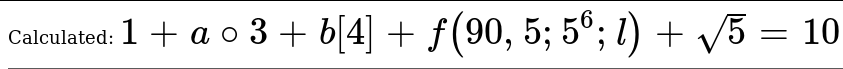
\includegraphics[scale=0.4]{screeenshot_SRS.png}
		\end{center}
	\end{frame}

	\begin{frame}
	\frametitle{How can we make it better?}
	\begin{itemize}
		\item Run-time changing for type of values
		\item Standart integral
		\item Arrays
		\item Better interface, smaller dependencies
		\item Operators with more than one symbols
		\item Convert codes to more programming languages
		\item Horner
		\item and other
	\end{itemize}
	\end{frame}

	\begin{frame}
		Special thanks for:
		\begin{itemize}
			\item ch. ace. Emil Kelevedjiev (BAS, \href{mailto:keleved@gmail.com}{keleved@gmail.com}, \href{http://keleved.com/}{http://keleved.com/})
			\item Todor Branzov (BAS)
			\item Konstantin Delchev (BAS, \href{http://kdelchev.com/}{http://kdelchev.com/})
			\item Konstantin Simeonov (Telerik a Progress company, \href{https://github.com/KonstantinSimeonov}{GitHub})
			\item Pano Panov (\href{mailto:pano.panov@gmail.com}{pano.panov@gmail.com}, \href{https://bg.linkedin.com/in/pano-panov-40357a75?trk=prof-samename-name}{LinkedIn})
		\end{itemize}
		\vspace{0.5cm}
		Acknowledges for:
		\begin{itemize}
			\item \href{http://www.math.bas.bg/omi/hssimi/}{High School Students Institute of Mathematics and Informatics}
			\item \href{http://www.math.bas.bg/}{Bulgarian Academy of Sciences}
			\item \href{http://www.smg.bg}{Sofia High School of Mathematics}
			\item \href{http://www.telerik.com}{Telerik a Progress Company}
		\end{itemize}
	\end{frame}
	
	\begin{frame}
	\frametitle{Resources}
		\begin{itemize}
			
			\item
			
				{\itshape GNU Compiler Collection}.\\ \texttt{https://gcc.gnu.org/}.\\ 
				Copyright \copyright\; 2009 Free Software Foundation, Inc.
			
			\item
			
				{\itshape MathJax}. \\ 
				\texttt{https://www.mathjax.org/}.\\
				Copyright \copyright\; 2015 The MathJax Consortium.
			
			\item
			
				{\itshape NeoVim (for demo)}. \\ 
				\texttt{https://neovim.io/}.\\
				Copyright \copyright\; Neovim contributors. All rights reserved.
			
			\item
			
				{\itshape Firefox (for demo)}. \\ 
				\texttt{https://mozilla.org/firefox}.\\
				Copyright \copyright\; Mozilla Foundation and contributors Mozilla Corporation.
			
		\end{itemize}
	\end{frame}
	
	\begin{frame}
		\begin{center}
			{\Huge Questions}
		\end{center}
	\end{frame}
	
	\begin{frame}
		\begin{center}
			{\Huge Thank you\\for\\the attention!}
		\end{center}
	\end{frame}

\end{document}
